

% \subsection{Planar Response of Cantilever Beam Under End Moment and End Force}\label{sec:plane}
\begin{figure}[H]
    \centering
    \ExampleFigure{frame-1001}
    \caption{Model for Example~\ref{sec:frame-1001}.}
    \label{fig:frame-1001}
\end{figure}
%
\subparagraph{Context.}
This example is selected to demonstrate the ability of the proposed formulations to accurately reproduce available analytical solutions through finite rotations.

\subparagraph{Setup.}
The cantilever beam  in Figure~\ref{fig:frame-1001} is subjected to a point moment \(\bm{M}\) at its free end \(\reflenx=L\). 
%
The centerline of the reference configuration 
is given by \(\bm{x}_0(\reflenx) = \reflenx\,\mathbf{E}_1\).
%

%
%
The configuration is expected
to remain in the \(\mathbf{E}_1 - \mathbf{E}_2\) plane.
Consequently, the out-of-plane director
\(\FrameBasis_3\) does not change during deformation so that \(\FrameBasis_3 \equiv \frameBasis_3\).
This simplification has two consequences:
\begin{itemize}
  \item There is no distinction between a spatially applied moment \(\bm{M} = M \, \frameBasis_3\)
    and a materially applied moment \(\bm{M} = M \, \FrameBasis_3\).
  \item The rotation \(\FrameRotation\) becomes
    vectorial, its variations \(\bm{u}_{\scriptscriptstyle{\Lambda}}^{(i)}\) at different configurations \(\chi^{(i)}\) can be added, and the sum of these variations over the course of global equilibrium iterations is equivalent
    to the logarithmic rotation increment:
    \[
      \sum_{i=0}^n \bm{u}_{\scriptscriptstyle{\Lambda}}^{(i)} \equiv \bm{\theta} 
     = \operatorname{Log} \left(\FrameRotation_{(n)}\FrameRotation_{(0)}^{\top}\right).
    \]
    %This is because the plane constraint has rendered the configuration manifold for \(\boldsymbol{\Lambda}\) vectorial.
\end{itemize}
%
In this case, the moment loading can be treated identically for all analyses by simply scaling a constant reference load vector for the node at \(\reflenx=L\):
%
\begin{equation}
  \mathbf{f}_{M,\text{ref}} = \begin{pmatrix}
     0 & 0 & M
  \end{pmatrix}^{\top}
  \label{eq:fref}
\end{equation}
%
where the reference magnitude \(M = \lambda 2 \pi EI/L \) varies with $\lambda=1/8, \ 1$, and $2$ for different cases causing the cantilever to loop over itself \(\lambda\) times. 
The following parameters are used:
\[
\begin{array}{lcr}
    L  &=&    10\hphantom{..}    \\ % ,& A  &= 1 \\
    E  &=&    10^4  \\ % ,& I  &= 10^{-2} \\
    G  &=&    10^4  \\ % ,& J  &= 10^{-2} \\
\end{array}
\qquad\qquad
\begin{array}{lcr}
    A  &=& 1\hphantom{..} \\
    I  &=& 10^{-2} \\
    J  &=& 10^{-2} \\
\end{array}
\]
The simulation uses a single load step with uniform meshes of 5 and 10 \ExactFrame{} elements. 
%
The solution requires only two iterations for each formulation matching the ideal performance reported by \cite{simo1986threedimensional}.
The tip displacements for the case \(\lambda = 1/8\) are collected in Table~\ref{tab:helical-plane} along with
the analytic solution of the governing boundary value problem in \eqref{eq:finite-equilibrium} given by:
\begin{equation*}
  \left\{
  \begin{aligned}
  \bm{x}(\reflenx)&=\frac{EI}{M} \sin \vartheta(\reflenx) \, \mathbf{E}_1
                      + \frac{EI}{M}\left(\cos \vartheta(\reflenx)-1\right) \, \mathbf{E}_2 \\
    \vartheta(\reflenx)   &=  \reflenx \frac{M}{EI}
  \end{aligned}
  \right.
\end{equation*}
%
where \(\vartheta\) parameterizes the rotation \(\FrameRotation(\reflenx) = \operatorname{Exp} \vartheta(\reflenx) \, \mathbf{E}_3\). 
% This result is derived in Appendix~\ref{sec:closed-solution}. 
The displacements for \(n=2\)-node elements match exactly those reported by \cite{ibrahimbegović1995computational} for both the natural \texttt{None}, and the logarithmic \texttt{Init}/\texttt{Incr} variants.
For \(n=3\)-node elements, the results match the analytic solution up to the reported precision.
%
%
\begin{center}
\begin{table}[H]
\caption{Tip displacements for the helical cantilever beam under $\lambda = 1/8$ for a discretization with 10 \(n\)-node elements.}
\label{tab:helical-plane}

% indicating agreement with exact solution (at M=2.75*loops, 2-nodes)

% indicating agreement with referenced formulations (at M=2.5, F=0.0625, 2-nodes)


\begin{tabular*}{\textwidth}{@{\extracolsep\fill}cccccccc@{}}
\toprule
\textbf{Interpolation} & \textbf{Isometry}  & \textbf{Parameters} & 
\(n\)  & \(\Delta x_1\) & \(\Delta x_2\) & \(\Delta x_3\)  \\
\midrule
% \texttt{None} & \texttt{None} & \texttt{None} & 2  & -0.994522 & 3.73019 & 0 \\
  \texttt{None} & \texttt{SFIN} & \texttt{None} & 2  & -0.994522 & 3.73019 & 0 \\
% \texttt{Incr} & \texttt{None} & \texttt{Incr} & 2  & -0.994522 & 3.73019 & 0 \\
  \texttt{Incr} & \texttt{SFIN} & \texttt{Incr} & 2  & -0.994522 & 3.73019 & 0 \\
% \texttt{Init} & \texttt{None} & \texttt{Init} & 2  & -0.994522 & 3.73019 & 0 \\
% \texttt{None} & \texttt{SFIN} & \texttt{Incr} & 2  & -0.994522 & 3.73019 & 0 \\
  \texttt{Incr} & \texttt{SFIN} & \texttt{None} & 2  & -0.994522 & 3.73019 & 0 \\
% \texttt{None} & \texttt{None} & \texttt{Incr} & 2  & -0.994522 & 3.73019 & 0 \\
%
  \hline
  \texttt{None} & \texttt{SFIN} & \texttt{None} & 3 & -0.996837 & 3.72923 & 0 \\
  \texttt{Incr} & \texttt{SFIN} & \texttt{Incr} & 3 & -0.996837 & 3.72923 & 0 \\ %-6.66134e-16
  \texttt{Incr} & \texttt{SFIN} & \texttt{None} & 3 & -0.996837 & 3.72923 & 0 \\ % -1.11022e-15 \\
\midrule
\textbf{Analytic} &             &               &   & \textbf{-0.996837} & \textbf{3.72923} & \textbf{0} \\ %-6.66134e-16
\hline
\end{tabular*}

\end{table}
\end{center}
%
%
\begin{figure}[H]
\centering
\begin{subfigure}[b]{0.48\textwidth}
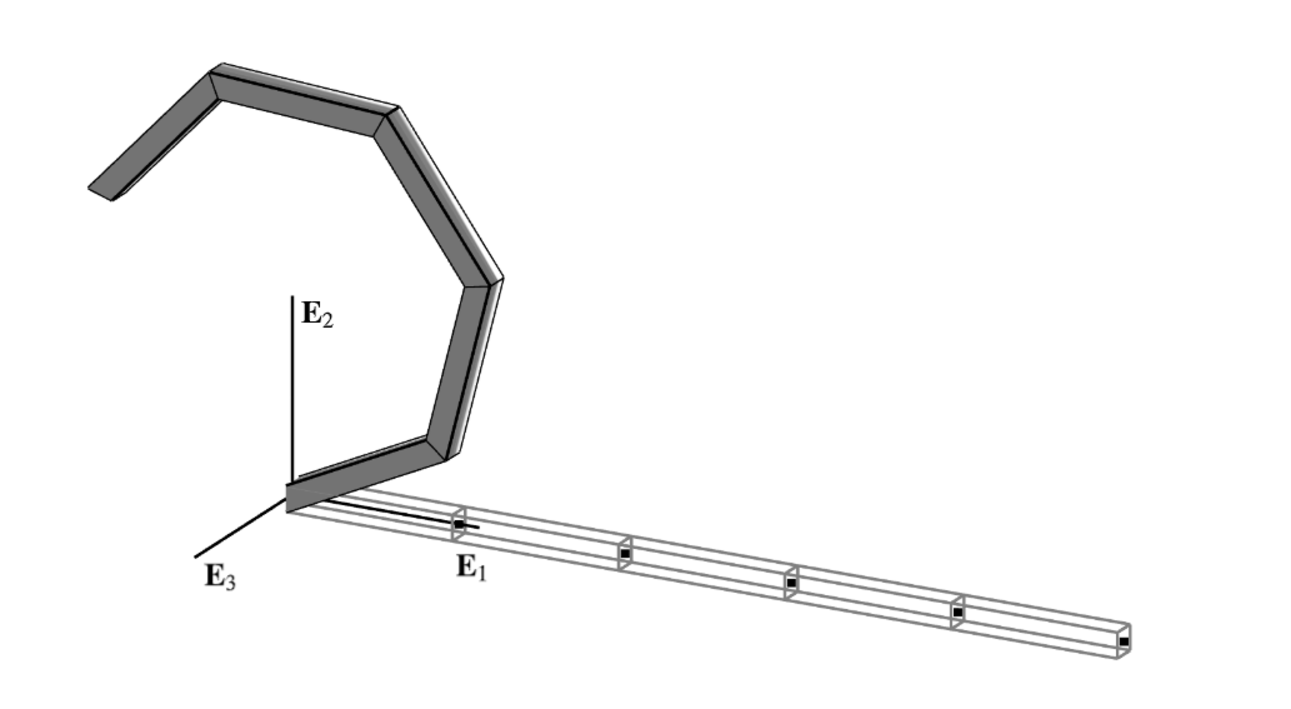
\includegraphics[width=0.7\textwidth,keepaspectratio]{Examples/frame-1001/Figures/Figure_1a}
  \caption{\(\lambda = 0.7\)}
  \label{fig:helical-a}
\end{subfigure}
\begin{subfigure}[b]{0.48\textwidth}
  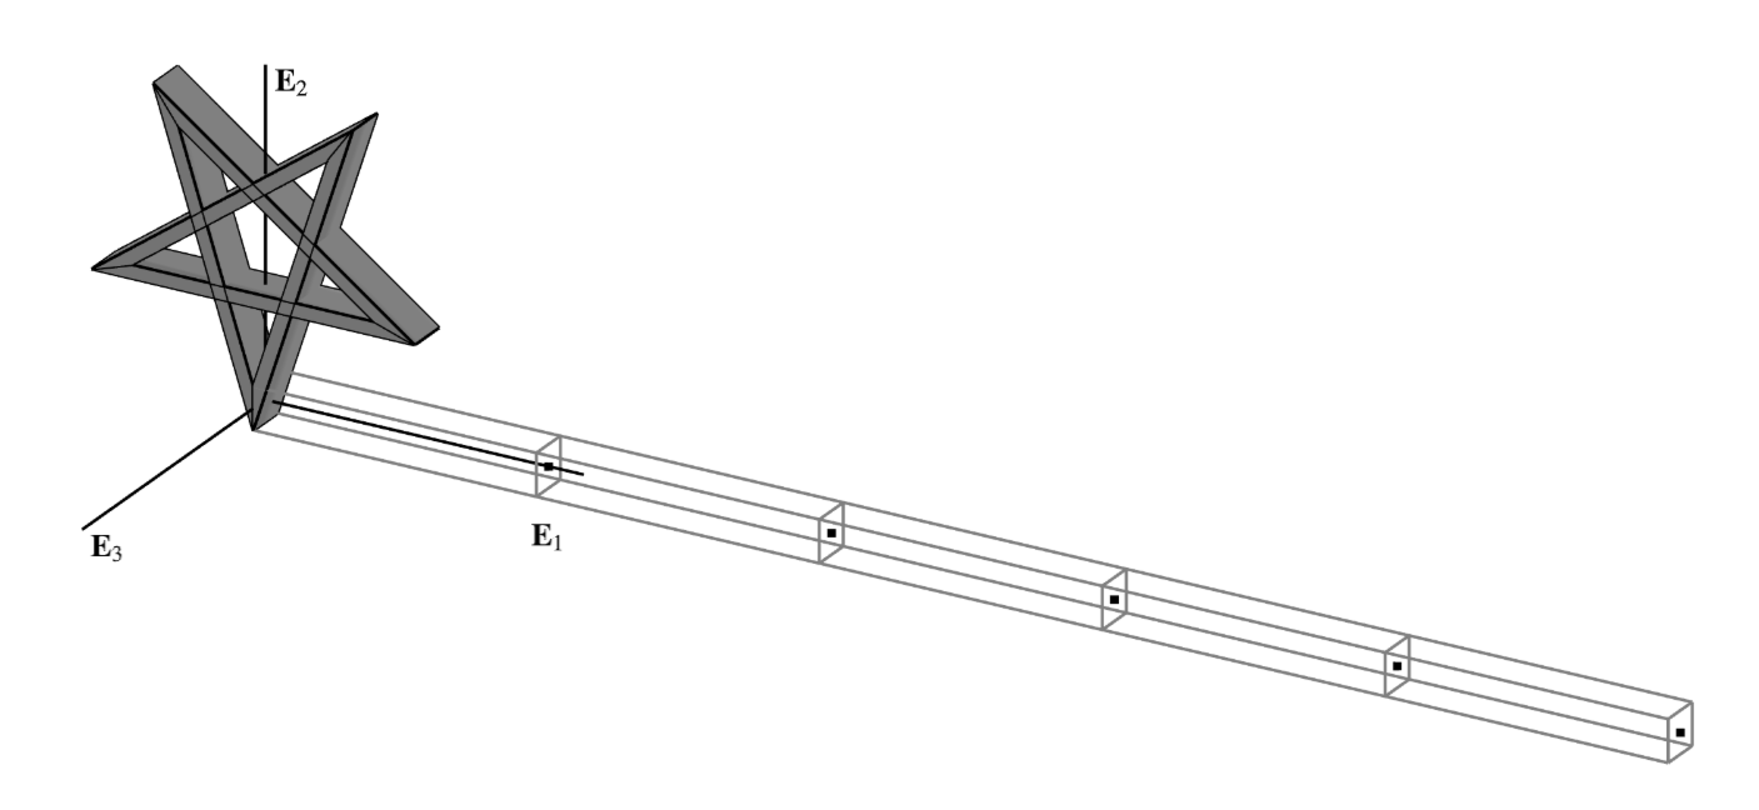
\includegraphics[width=0.8\textwidth,keepaspectratio]{Examples/frame-1001/Figures/Figure_1b}
  \caption{\(\lambda = 2\)}
  \label{fig:helical-b}
\end{subfigure}
\caption{Deformed configuration of cantilever beam under two moment magnitudes.}
\label{fig:cantilever-1001}
\end{figure}